%Version 3.1 December 2024
% See section 11 of the User Manual for version history
%
%%%%%%%%%%%%%%%%%%%%%%%%%%%%%%%%%%%%%%%%%%%%%%%%%%%%%%%%%%%%%%%%%%%%%%
%%                                                                 %%
%% Please do not use \input{...} to include other tex files.       %%
%% Submit your LaTeX manuscript as one .tex document.              %%
%%                                                                 %%
%% All additional figures and files should be attached             %%
%% separately and not embedded in the \TeX\ document itself.       %%
%%                                                                 %%
%%%%%%%%%%%%%%%%%%%%%%%%%%%%%%%%%%%%%%%%%%%%%%%%%%%%%%%%%%%%%%%%%%%%%

%%\documentclass[referee,sn-basic]{sn-jnl}% referee option is meant for double line spacing

%%=======================================================%%
%% to print line numbers in the margin use lineno option %%
%%=======================================================%%

%%\documentclass[lineno,pdflatex,sn-basic]{sn-jnl}% Basic Springer Nature Reference Style/Chemistry Reference Style

%%=========================================================================================%%
%% the documentclass is set to pdflatex as default. You can delete it if not appropriate.  %%
%%=========================================================================================%%

%%\documentclass[sn-basic]{sn-jnl}% Basic Springer Nature Reference Style/Chemistry Reference Style

%%Note: the following reference styles support Namedate and Numbered referencing. By default the style follows the most common style. To switch between the options you can add or remove “Numbered” in the optional parenthesis. 
%%The option is available for: sn-basic.bst, sn-chicago.bst%  
 
%%\documentclass[pdflatex,sn-nature]{sn-jnl}% Style for submissions to Nature Portfolio journals
%%\documentclass[pdflatex,sn-basic]{sn-jnl}% Basic Springer Nature Reference Style/Chemistry Reference Style
% The float package is loaded before the class: the class loads hyperref, and a float package loaded
% after hyperref (by the algorithm package below) writes the anchor of every figure and algorithm twice.
\RequirePackage{float}
\documentclass[pdflatex,sn-mathphys-num]{sn-jnl}% Math and Physical Sciences Numbered Reference Style
%%\documentclass[pdflatex,sn-mathphys-ay]{sn-jnl}% Math and Physical Sciences Author Year Reference Style
%%\documentclass[pdflatex,sn-aps]{sn-jnl}% American Physical Society (APS) Reference Style
%%\documentclass[pdflatex,sn-vancouver-num]{sn-jnl}% Vancouver Numbered Reference Style
%%\documentclass[pdflatex,sn-vancouver-ay]{sn-jnl}% Vancouver Author Year Reference Style
%%\documentclass[pdflatex,sn-apa]{sn-jnl}% APA Reference Style
%%\documentclass[pdflatex,sn-chicago]{sn-jnl}% Chicago-based Humanities Reference Style

%%%% Standard Packages
%%<additional latex packages if required can be included here>
\usepackage[T1]{fontenc}

\usepackage{graphicx}%
\usepackage{multirow}%
\usepackage{amsmath,amssymb,amsfonts}%
\usepackage{amsthm}%
\usepackage{mathrsfs}%
\usepackage[title]{appendix}%
\usepackage{xcolor}%
\usepackage{textcomp}%
\usepackage{manyfoot}%
\usepackage{booktabs}%
\usepackage{algorithm}%
\usepackage{algorithmicx}%
\usepackage{algpseudocode}%
\usepackage{listings}%
%%%%
% References by \cref. With \newtheorem and a shared counter, \cref calls a lemma "Theorem" under this class,
% so the environments that share the counter of theorem are declared with thmtools below.
\usepackage{thmtools}%
\usepackage[capitalise,noabbrev]{cleveref}%

%%%%%=============================================================================%%%%
%%%%  Remarks: This template is provided to aid authors with the preparation
%%%%  of original research articles intended for submission to journals published 
%%%%  by Springer Nature. The guidance has been prepared in partnership with 
%%%%  production teams to conform to Springer Nature technical requirements. 
%%%%  Editorial and presentation requirements differ among journal portfolios and 
%%%%  research disciplines. You may find sections in this template are irrelevant 
%%%%  to your work and are empowered to omit any such section if allowed by the 
%%%%  journal you intend to submit to. The submission guidelines and policies 
%%%%  of the journal take precedence. A detailed User Manual is available in the 
%%%%  template package for technical guidance.
%%%%%=============================================================================%%%%

%% as per the requirement new theorem styles can be included as shown below
\theoremstyle{thmstyleone}%
\newtheorem{theorem}{Theorem}%  meant for continuous numbers
%%\newtheorem{theorem}{Theorem}[section]% meant for sectionwise numbers
%% optional argument [theorem] produces theorem numbering sequence instead of independent numbers for Proposition
%%\newtheorem{proposition}[theorem]{Proposition}%
%%\newtheorem{proposition}{Proposition}% to get separate numbers for theorem and proposition etc.
% Proposition, Lemma and Corollary are numbered with Theorem, in the style of Theorem.
\declaretheorem[name=Proposition, style=thmstyleone, sibling=theorem]{proposition}%
\declaretheorem[name=Lemma, style=thmstyleone, sibling=theorem]{lemma}%
\declaretheorem[name=Corollary, style=thmstyleone, sibling=theorem]{corollary}%

\theoremstyle{thmstyletwo}%
\newtheorem{example}{Example}%
\newtheorem{remark}{Remark}%

\theoremstyle{thmstylethree}%
\newtheorem{definition}{Definition}%

% Algorithm: the input and the output are headed "Input:" and "Output:".
\algrenewcommand\algorithmicrequire{\textbf{Input:}}%
\algrenewcommand\algorithmicensure{\textbf{Output:}}%

% Notation.
\newcommand{\cp}{\operatorname{cp}}% cp(u,v): number of edges of a minimum cut-path
\newcommand{\DC}{\mathcal{DC}_2}% graphs with distance or cut-value at most two
\newcommand{\MinCutPath}{\textsc{Min Cut-Path}}%
\newcommand{\SSP}{\textsc{Separating Shortest Path}}%

% Title and author of the PDF file.
\hypersetup{pdftitle={Min Cut-Path on Graphs with Distance or Cut-Value at Most Two}, pdfauthor={Norbert Miche\v{l}}}%

\raggedbottom
%%\unnumbered% uncomment this for unnumbered level heads

\begin{document}

\title{Min Cut-Path on Graphs with Distance or Cut-Value at Most Two}

%%=============================================================%%
%% GivenName	-> \fnm{Joergen W.}
%% Particle	-> \spfx{van der} -> surname prefix
%% FamilyName	-> \sur{Ploeg}
%% Suffix	-> \sfx{IV}
%% \author*[1,2]{\fnm{Joergen W.} \spfx{van der} \sur{Ploeg} 
%%  \sfx{IV}}\email{iauthor@gmail.com}
%%=============================================================%%

\author*{\fnm{Norbert} \sur{Miche\v{l}}}\email{5344553@upjs.sk}

\affil{\orgdiv{Institute of Computer Science, Faculty of Science}, \orgname{Pavol Jozef \v{S}af\'arik University in Ko\v{s}ice}, \orgaddress{\street{Jesenn\'a 5}, \city{Ko\v{s}ice}, \postcode{040 01}, \country{Slovakia}}}

%%==================================%%
%% Sample for unstructured abstract %%
%%==================================%%

\abstract{A cut-path between two vertices $u$ and $v$ of a graph is a set of edges that contains both a $u$--$v$ path and a cut separating $u$ from $v$.
The \MinCutPath{} problem asks for a cut-path with the fewest edges.
Let $d(u,v)$ be the distance between $u$ and $v$, and let the cut-value $c(u,v)$ be the size of a minimum cut separating them.
For a pair with $c(u,v) = 2$, a minimum cut-path has $d(u,v)$ or $d(u,v) + 1$ edges, and we characterize the first case in arbitrary graphs.
The minimum cuts between $u$ and $v$ divide the graph into a chain of subgraphs.
A minimum cut-path has $d(u,v)$ edges if and only if one of these subgraphs contains a path that is part of a shortest $u$--$v$ path and separates two prescribed vertices of the subgraph.
We apply this criterion to the graphs in which every two vertices are at distance at most two or have cut-value at most two, a class that contains the graphs of diameter two and the cactus graphs.
In such a graph, a minimum cut-path is computed in linear time for every pair with cut-value at most two, in particular for every pair at distance at least three.
On any other graph, the same algorithm returns a minimum cut-path or two vertices whose distance and cut-value are both at least three.
In general graphs, deciding whether a minimum cut-path has $d(u,v)$ edges is NP-complete already for pairs with $c(u,v) = 2$.
In the class, the pairs at distance two with cut-value at least three remain open.}

%%================================%%
%% Sample for structured abstract %%
%%================================%%

% \abstract{\textbf{Purpose:} The abstract serves both as a general introduction to the topic and as a brief, non-technical summary of the main results and their implications. The abstract must not include subheadings (unless expressly permitted in the journal's Instructions to Authors), equations or citations. As a guide the abstract should not exceed 200 words. Most journals do not set a hard limit however authors are advised to check the author instructions for the journal they are submitting to.
% 
% \textbf{Methods:} The abstract serves both as a general introduction to the topic and as a brief, non-technical summary of the main results and their implications. The abstract must not include subheadings (unless expressly permitted in the journal's Instructions to Authors), equations or citations. As a guide the abstract should not exceed 200 words. Most journals do not set a hard limit however authors are advised to check the author instructions for the journal they are submitting to.
% 
% \textbf{Results:} The abstract serves both as a general introduction to the topic and as a brief, non-technical summary of the main results and their implications. The abstract must not include subheadings (unless expressly permitted in the journal's Instructions to Authors), equations or citations. As a guide the abstract should not exceed 200 words. Most journals do not set a hard limit however authors are advised to check the author instructions for the journal they are submitting to.
% 
% \textbf{Conclusion:} The abstract serves both as a general introduction to the topic and as a brief, non-technical summary of the main results and their implications. The abstract must not include subheadings (unless expressly permitted in the journal's Instructions to Authors), equations or citations. As a guide the abstract should not exceed 200 words. Most journals do not set a hard limit however authors are advised to check the author instructions for the journal they are submitting to.}

\keywords{Separating shortest path, Edge connectivity, Minimum cuts, Linear-time algorithm, NP-completeness}

%%\pacs[JEL Classification]{D8, H51}

%%\pacs[MSC Classification]{35A01, 65L10, 65L12, 65L20, 65L70}

\maketitle

\section{Introduction}\label{sec:introduction}

Let $G$ be a connected graph, and let $u$ and $v$ be two distinct vertices of $G$.
A \emph{cut-path} between $u$ and $v$ is a set of edges that contains a $u$--$v$ path and a cut separating $u$ from $v$.
The \MinCutPath{} problem asks for a cut-path with the fewest edges, and $\cp(u, v)$ denotes their number.
Let $d(u, v)$ be the distance between $u$ and $v$, and let the cut-value $c(u, v)$ be the minimum number of edges of a cut separating $u$ from $v$.
The union of a minimum cut and a shortest path is a cut-path, and the two share an edge, which gives the upper bound in
\[
\max\{c(u, v), d(u, v)\} \leq \cp(u, v) \leq c(u, v) + d(u, v) - 1
\]
(\cref{lem:basic-bounds}).

The \MinCutPath{} problem was introduced in the author's master's thesis~\cite{Michel2025MinCutPath}.
The upper bound is attained by all pairs of vertices in graphs of diameter two and in cactus graphs~\cite[Theorems~15 and~18]{Michel2025MinCutPath}, where the cactus graphs are the connected graphs with $c(x, y) \leq 2$ for all pairs $x, y$ (\cref{sec:class}).
A shortest $u$--$v$ path is separating if the removal of its edges separates $u$ from $v$, and $\cp(u, v) = d(u, v)$ if and only if such a path exists.
Deciding whether it exists, the \SSP{} problem, is NP-complete~\cite[Theorem~3.10]{Michel2026MinCutPath}.

The formula $\cp(u, v) = c(u, v) + d(u, v) - 1$ fails if every pair of vertices is required to satisfy only one of the two hypotheses.
Let $\DC$ be the class of connected graphs in which every two distinct vertices $x$ and $y$ satisfy $d(x, y) \leq 2$ or $c(x, y) \leq 2$.
The thesis defines this class and gives two graphs in it with $\cp(u, v) = 3$ and $c(u, v) + d(u, v) - 1 = 4$~\cite[Definition~37 and Figure~3.3]{Michel2025MinCutPath}.
In a graph of $\DC$, the formula holds for the pairs with $d(u, v) = 1$ or $c(u, v) = 1$, and two kinds of pairs remain (\cref{prop:easy-pairs}).
A pair with $c(u, v) = 2$ has $\cp(u, v) \in \{d(u, v), d(u, v) + 1\}$, and a pair with $d(u, v) = 2$ and $c(u, v) \geq 3$ has $\cp(u, v) \in \{c(u, v), c(u, v) + 1\}$.
We compute a minimum cut-path for the pairs of the first kind in linear time, and we prove that the same task is NP-hard without the hypothesis $G \in \DC$.

\subsection{Related Work}\label{sec:related-work}

By Menger's theorem, $c(u, v)$ is the maximum number of pairwise edge-disjoint $u$--$v$ paths~\cite[Corollary~3.3.5]{Diestel2025}.
Picard and Queyranne~\cite{PicardQueyranne1980} described all minimum cuts between two vertices of a network by one maximum flow.
A set that contains the source and not the sink is the source side of a minimum cut if and only if no arc of the residual digraph leaves it.
For an undirected graph, contract every class of vertices that no minimum $u$--$v$ cut separates and direct the remaining edges along a maximum flow.
The result is an acyclic digraph in which every vertex other than the classes of $u$ and $v$ has as many entering as leaving edges, a structure that Dinitz and Vainshtein call a strip (see~\cite{BaswanaPandey2025Carcass}).
All minimum cuts of a graph are represented by a cactus, a result of Dinits, Karzanov and Lomonosov (see~\cite{NagamochiKameda1996}).
For a 2-edge-connected graph that is not 3-edge-connected, this cactus is obtained by contracting every 3-edge-connected component, that is, every class of the relation $c(x, y) \geq 3$, and it is computed in linear time~\cite{Mehlhorn2017Certifying}.
For a pair with $c(u, v) = 2$, the square decomposition of \cref{sec:structure} is an explicit form of these representations.
We prove its properties directly, because \cref{sec:separating,sec:algorithm} use the terminals of the squares and distances inside the squares, which a contraction does not keep.

A $u$--$v$ path is non-disconnecting if the removal of its edges leaves the graph connected.
Deciding whether such a path exists is NP-hard~\cite{Mao2021NonSeparating}, and a shortest one is found in FPT time with respect to its length~\cite{Abhinav2022NonSeparating}.
For two pairs of vertices, it is NP-complete to decide whether some shortest path between the first pair is edge-disjoint from some path between the second pair~\cite{EilamTzoreff1998Disjoint}.
\SSP{} asks the opposite, namely whether the removal of the edges of some shortest $u$--$v$ path separates $u$ from $v$.

Graphs in which the local edge-connectivity $c(x, y)$ of every pair of vertices is at most a constant $k$ were studied for coloring problems~\cite{Aboulker2017Coloring}.
For $k = 2$ the connected graphs of this kind are the cactus graphs.
The class $\DC$ asks for $c(x, y) \leq 2$ only when $d(x, y) \geq 3$, so it contains all cactus graphs and all connected graphs of diameter two.
To the best of our knowledge, a class defined by such a condition on distances and cut-values has not been studied.
Graphs of diameter two are also a polynomial case of \textsc{Matching Cut} and, for unit edge lengths, of \textsc{Shortest Path Most Vital Edges}, and both problems are NP-hard on graphs of diameter three~\cite{LeLe2019MatchingCut,Bazgan2019MostVital}.

\subsection{Our Results}\label{sec:results}

\begin{enumerate}
\item \emph{A characterization for cut-value two.}
Let $c(u, v) = 2$ in an arbitrary connected graph.
The minimum $u$--$v$ cuts divide the graph into a chain of subgraphs, the squares, and every $u$--$v$ path enters and leaves each square at one of at most four vertices of the square, its terminals (\cref{thm:structure}).
We prove that $\cp(u, v) = d(u, v)$ if and only if some square contains a path of the following kind (\cref{thm:characterization}).
The path leads from an entering terminal to a leaving terminal, it is part of a shortest $u$--$v$ path, and it separates the other entering terminal from the other leaving terminal in the square.
Otherwise $\cp(u, v) = d(u, v) + 1$.

\item \emph{Linear time in the class $\DC$.}
We give an algorithm that, for a graph $G = (V, E)$ of $\DC$ and two vertices $u$ and $v$, decides in $O(|V| + |E|)$ time whether $c(u, v) \leq 2$ and, if so, computes $\cp(u, v)$ and a minimum cut-path (\cref{thm:linear-time}).
The algorithm does not test whether $G \in \DC$, and for a connected graph outside the class it returns the same or two vertices $x, y$ with $c(x, y) \geq 3$ and $d(x, y) \geq 3$.
The running time includes the computation of the squares.
In a graph of $\DC$, every pair with $d(u, v) \geq 3$ has $c(u, v) \leq 2$ and is solved in this way, and a pair with $d(u, v) = 1$ is solved by one computation of a minimum cut (\cref{cor:class-pairs}).

\item \emph{NP-completeness for cut-value two.}
We prove that, in general graphs, deciding whether $\cp(u, v) = d(u, v)$ is NP-complete already for pairs with $c(u, v) = 2$ (\cref{thm:hardness}).
Hence, unless $\mathrm{P} = \mathrm{NP}$, no polynomial-time algorithm computes $\cp(u, v)$ for all such pairs, and the second outcome of the previous item cannot be avoided.
For the cut-value, this theorem answers the question of~\cite{Michel2026MinCutPath} about the complexity of \MinCutPath{} for bounded $c(u, v)$.

\item \emph{Pairs at distance two.}
In a graph of $\DC$, the pairs with $d(u, v) = 2$ and $c(u, v) \geq 3$ are the only pairs that we do not solve.
We show that such a pair has $\cp(u, v) = c(u, v)$ if and only if some minimum $u$--$v$ cut contains a $u$--$v$ path (\cref{prop:open-pairs}).
\end{enumerate}

\subsection{Techniques}\label{sec:techniques}

The square decomposition reduces the question whether a $u$--$v$ path $R$ separates $u$ from $v$ to the squares.
Consecutive squares are joined by two general paths, which consist of the edges of the minimum cuts and of further subgraphs, the links, and $R$ follows exactly one of them (\cref{thm:structure}).
The other general path remains in $G \setminus R$ and joins the terminals of the two squares that $R$ does not use.
Hence $u$ and $v$ are separated in $G \setminus R$ if and only if, in some square, the part of $R$ in the square separates the entering terminal that $R$ does not use from the leaving terminal that $R$ does not use (\cref{lem:criterion}).
We call this part the trace of $R$ in the square.

In a graph of $\DC$, the trace of a shortest $u$--$v$ path has at most two edges.
Two distinct terminals of a square have cut-value at least three (\cref{thm:structure}(v)), so they are at distance at most two by the definition of the class, and the trace is a shortest path between two terminals (\cref{cor:two-edges}).
A trace with one edge is determined by its ends.
A trace $x, w, y$ that separates the other two terminals shares an edge with any fixed path $q$ of the square between them, so $xw$ or $wy$ is an edge of $q$, which leaves at most four candidates.
Every square is therefore examined by a constant number of graph searches, and the squares are pairwise disjoint.
In an arbitrary graph, two terminals between which a trace would need at least three edges have distance and cut-value at least three, and the algorithm returns them if it finds no separating trace with at most two edges.
The squares are computed from two edge-disjoint $u$--$v$ paths, because an edge of these paths lies in a minimum $u$--$v$ cut if and only if its ends lie in different strong components of the residual graph (\cref{lem:residual}).

For \cref{thm:hardness}, we join a new vertex $u'$ to $u$ by two paths of length two.
The pair $u', v$ has cut-value two, and if $c(u, v) \geq 3$, the original graph is one square with the terminals $u$ and $v$.
Every connected graph with a pair of cut-value at least three thus occurs as a square if the distances between the terminals are not bounded.

\subsection{Relation to the Thesis}\label{sec:thesis}

This paper is based on Section~3.3 of the thesis~\cite{Michel2025MinCutPath}.
The class $\DC$, the two graphs of \cref{ex:counterexamples}, the notions of a square and of a general path, and the idea of a polynomial and of a linear-time algorithm for pairs with cut-value two are taken from there~\cite[Definitions~37 to~40 and Theorems~20, 22 and~23]{Michel2025MinCutPath}.
The thesis obtains a decomposition by three transformations of the graph.
Here the decomposition is defined by the union of all minimum $u$--$v$ cuts, and every statement has a complete proof.
The separation criterion and the characterization for arbitrary graphs (\cref{lem:criterion,thm:characterization}), the linear running time that includes the computation of the decomposition (\cref{thm:linear-time}) and the NP-completeness for cut-value two (\cref{thm:hardness}) are new.

\section{Preliminaries}
\label{sec:preliminaries}

\subsection{Cut-Paths and Minimum Cuts}
\label{sec:cut-paths}

All graphs are finite, simple and undirected.
Notions that are not defined here follow~\cite{Diestel2025}.
Throughout the paper, $G = (V, E)$ is a connected graph, and $u$ and $v$ are two distinct vertices of $G$.
We write $xy$ for the edge with the ends $x$ and $y$.
A path is a sequence of distinct vertices in which consecutive vertices are adjacent, and a single vertex is a path with no edges.
A path from $x$ to $y$ is an $x$--$y$ path.
We write $|P|$ for the number of edges of a path $P$ and use the symbol $P$ also for the set of its edges.
The distance $d(x, y)$ is the number of edges of a shortest $x$--$y$ path of $G$.
For a subgraph $H$ of $G$ and a set $M \subseteq E$, the graph $H \setminus M$ is obtained from $H$ by removing the edges of $M$.

Let $x$ and $y$ be two distinct vertices.
A set $C \subseteq E$ is an \emph{$x$--$y$ cut} if $G \setminus C$ contains no $x$--$y$ path.
The minimum size of an $x$--$y$ cut is the \emph{cut-value} $c(x, y)$.
For a set $A \subseteq V$, we denote by $\delta(A)$ the set of all edges with exactly one end in $A$.
If $x \in A$ and $y \notin A$, then $\delta(A)$ is an $x$--$y$ cut.
Distances and cut-values in a subgraph $H$ are written $d_H$ and $c_H$.

\begin{definition}[Cut-path]
\label{def:cut-path}
A \emph{cut-path} between $u$ and $v$ is a set of edges of $G$ that contains a $u$--$v$ path and a $u$--$v$ cut.
The minimum number of edges of a cut-path between $u$ and $v$ is denoted by $\cp(u, v)$, and a cut-path with $\cp(u, v)$ edges is a \emph{minimum cut-path}.
\end{definition}

The \MinCutPath{} problem asks for a minimum cut-path between $u$ and $v$~\cite{Michel2025MinCutPath}.
A shortest $u$--$v$ path $P$ is \emph{separating} if $G \setminus P$ contains no $u$--$v$ path, and the \SSP{} problem asks whether $G$ contains such a path.
The two bounds of \cref{lem:basic-bounds} are those of~\cite[Claim~7]{Michel2025MinCutPath}, and we include the short proof.

\begin{lemma}[Basic bounds]
\label{lem:basic-bounds}
The value $\cp(u, v)$ satisfies
\[
\max\{c(u, v), d(u, v)\} \leq \cp(u, v) \leq c(u, v) + d(u, v) - 1.
\]
The equality $\cp(u, v) = d(u, v)$ holds if and only if $G$ contains a separating shortest $u$--$v$ path.
\end{lemma}

\begin{proof}
A cut-path contains a $u$--$v$ cut and a $u$--$v$ path, which gives the lower bound.
A shortest $u$--$v$ path $P$ shares an edge with every minimum $u$--$v$ cut $C$, so $C \cup P$ is a cut-path with at most $c(u, v) + d(u, v) - 1$ edges.
A separating shortest $u$--$v$ path is a $u$--$v$ cut, hence a cut-path with $d(u, v)$ edges.
Conversely, a cut-path with $d(u, v)$ edges contains a $u$--$v$ path, which has at least $d(u, v)$ edges.
The cut-path is therefore equal to this path, which is a shortest $u$--$v$ path and a $u$--$v$ cut.
\end{proof}

\begin{lemma}
\label{lem:minimum-cuts}
Let $C$ be a minimum $u$--$v$ cut.
Then $G \setminus C$ has exactly two components, and $C = \delta(A)$ for exactly one set $A \subseteq V$ with $u \in A$, the vertex set of the component that contains $u$.
For every set $A \subseteq V$ with $u \in A$ and $v \notin A$, every $u$--$v$ path contains an odd number of edges of $\delta(A)$.
\end{lemma}

\begin{proof}
Let $A$ be the vertex set of the component of $G \setminus C$ that contains $u$.
Every edge of $\delta(A)$ belongs to $C$, and $\delta(A)$ is a $u$--$v$ cut because $v \notin A$.
Hence $\delta(A) = C$ by the minimality of $C$.
Let $Y$ be the component of $G \setminus C$ that contains $v$, and suppose that there is a third component $Y'$.
Since $G$ is connected, some edge of $G$ has exactly one end in $Y'$.
This edge belongs to $C = \delta(A)$ and has no end in $Y$.
The edges of $C$ with an end in $Y$ thus form a $u$--$v$ cut with fewer than $|C|$ edges, a contradiction.
If $C = \delta(A')$ for a set $A'$ with $u \in A'$, then no edge of $G \setminus C$ has exactly one end in $A'$, so $A'$ is the union of the vertex sets of some components of $G \setminus C$.
Since $\delta(V)$ is empty and $C$ is not, we have $A' \neq V$ and hence $A' = A$.

For the last statement, follow a $u$--$v$ path from $u$ to $v$.
The path changes between $A$ and $V \setminus A$ exactly at its edges in $\delta(A)$, it starts in $A$ and it ends outside $A$.
\end{proof}

When we write a minimum $u$--$v$ cut as $\delta(A)$, the set $A$ contains $u$.

\begin{lemma}
\label{lem:uncrossing}
Let $A, B \subseteq V$, and let $m(A, B)$ be the number of edges with one end in $A \setminus B$ and the other end in $B \setminus A$.
Then
\[
|\delta(A \cap B)| + |\delta(A \cup B)| = |\delta(A)| + |\delta(B)| - 2m(A, B).
\]
\end{lemma}

\begin{proof}
The sets $A \cap B$, $A \setminus B$, $B \setminus A$ and $V \setminus (A \cup B)$ partition $V$.
An edge with both ends in one of them is counted on neither side.
An edge between $A \setminus B$ and $B \setminus A$ belongs to $\delta(A)$ and to $\delta(B)$ and to neither set on the left-hand side.
An edge between $A \cap B$ and $V \setminus (A \cup B)$ belongs to all four sets.
Every other edge belongs to exactly one of $\delta(A)$, $\delta(B)$ and to exactly one of $\delta(A \cap B)$, $\delta(A \cup B)$.
\end{proof}

The inequality $|\delta(A \cap B)| + |\delta(A \cup B)| \leq |\delta(A)| + |\delta(B)|$ is the submodularity of the cut function.

\subsection{Graphs with Distance or Cut-Value at Most Two}
\label{sec:class}

\begin{definition}[The class $\DC$, {\cite[Definition~37]{Michel2025MinCutPath}}]
\label{def:class}
The class $\DC$ consists of all connected graphs in which every two distinct vertices $x$ and $y$ satisfy $d(x, y) \leq 2$ or $c(x, y) \leq 2$.
\end{definition}

A graph has \emph{diameter at most two} if any two of its vertices are at distance at most two.
A \emph{cactus graph} is a connected graph in which any two distinct cycles share at most one vertex.
The cactus graphs are the connected graphs in which $c(x, y) \leq 2$ for every two distinct vertices $x$ and $y$.
This characterization is folklore (one direction is proved in~\cite[Claim~17]{Michel2025MinCutPath}, both in~\cite[Lemma~6.1]{Michel2026MinCutPath}).

\begin{proposition}
\label{prop:class}
The relation on $V$ that holds for $x$ and $y$ if $x = y$ or $c(x, y) \geq 3$ is an equivalence relation.
The graph $G$ belongs to $\DC$ if and only if any two vertices of the same equivalence class are at distance at most two in $G$.
In particular, $\DC$ contains all connected graphs of diameter at most two and all cactus graphs.
\end{proposition}

\begin{proof}
The relation is reflexive and symmetric.
For transitivity, let $x, y, z$ be distinct vertices with $c(x, y) \geq 3$ and $c(y, z) \geq 3$, and let $C$ be a minimum $x$--$z$ cut.
If $y$ lies in the component of $G \setminus C$ that contains $x$, then $C$ is a $y$--$z$ cut, and otherwise $C$ is an $x$--$y$ cut.
In both cases $|C| \geq 3$.
By \cref{def:class}, the graph $G$ lies outside $\DC$ if and only if some two distinct vertices $x, y$ satisfy $c(x, y) \geq 3$ and $d(x, y) \geq 3$, which is the second statement.
In a graph of diameter at most two all distances are at most two, and in a cactus graph every equivalence class is a single vertex.
\end{proof}

The equivalence classes of \cref{prop:class} are called 3-edge-connected components in~\cite{Mehlhorn2017Certifying}, where they are computed in linear time.

In graphs of diameter at most two and in cactus graphs, every pair satisfies $\cp(u, v) = c(u, v) + d(u, v) - 1$~\cite[Theorems~15 and~18]{Michel2025MinCutPath}.
\Cref{fig:graph-classes} shows the three classes.
The formula fails in $\DC$, as the two graphs of~\cite[Figure~3.3]{Michel2025MinCutPath} show (\cref{ex:counterexamples}).

\begin{figure}[tb]
    \centering
    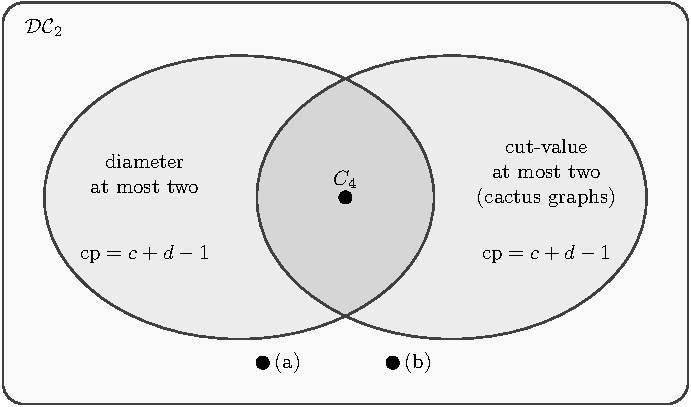
\includegraphics{graph-classes.pdf}
    \caption{The class $\DC$ and its two subclasses; (a) and (b) are the graphs $G_a$ and $G_b$ of \cref{fig:counterexamples}}
    \label{fig:graph-classes}
\end{figure}

\begin{example}
\label{ex:counterexamples}
Let $G_a$ be the graph with the vertices $u, v, a, b, s, t$ and the edges $ua$, $us$, $sb$, $ab$, $at$, $tv$, $bv$, and let $G_b$ be obtained from $G_a$ by adding the edges $av$ and $ub$ (\cref{fig:counterexamples}).
In both graphs, the removal of the path $u, a, b, v$ leaves the components $\{u, s, b\}$ and $\{a, t, v\}$, so this path is a cut-path with three edges.
In $G_a$ we have $c(u, v) = 2$ and $d(u, v) = 3$, and in $G_b$ we have $c(u, v) = 3$ and $d(u, v) = 2$.
Hence $\cp(u, v) = 3$ in both graphs by \cref{lem:basic-bounds}, whereas $c(u, v) + d(u, v) - 1 = 4$.
Both graphs belong to $\DC$.
In $G_a$ the only two vertices of degree greater than two are $a$ and $b$, which are adjacent.
In $G_b$ the only two vertices at distance three are $s$ and $t$, which have degree two.
Neither graph has diameter two, and neither is a cactus graph.
\end{example}

\begin{figure}[tb]
    \centering
    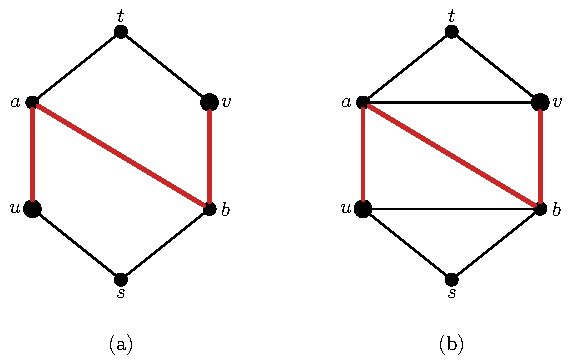
\includegraphics{counterexamples.pdf}
    \caption{The graphs $G_a$ (a) and $G_b$ (b) of \cref{ex:counterexamples}; the cut-path $u, a, b, v$ is red}
    \label{fig:counterexamples}
\end{figure}

\begin{proposition}
\label{prop:easy-pairs}
(i) If $d(u, v) = 1$, then $\cp(u, v) = c(u, v)$, and every minimum $u$--$v$ cut is a minimum cut-path.
(ii) If $c(u, v) = 1$, then $\cp(u, v) = d(u, v)$, and every shortest $u$--$v$ path is a minimum cut-path.
(iii) If $c(u, v) = 2$, then $\cp(u, v) \in \{d(u, v), d(u, v) + 1\}$.
(iv) If $d(u, v) = 2$, then $\cp(u, v) \in \{c(u, v), c(u, v) + 1\}$.
If $G \in \DC$, then $d(u, v) \leq 2$ or $c(u, v) \leq 2$, so at least one of the four statements applies to every pair $u, v$.
\end{proposition}

\begin{proof}
The four values follow from \cref{lem:basic-bounds}.
If $d(u, v) = 1$, the edge $uv$ is a $u$--$v$ path and lies in every $u$--$v$ cut, so every minimum $u$--$v$ cut is a cut-path.
If $c(u, v) = 1$, the edge of a $u$--$v$ cut of size one lies on every $u$--$v$ path, so every shortest $u$--$v$ path is a cut-path.
The last statement is \cref{def:class}.
\end{proof}

By \cref{prop:easy-pairs}, a minimum cut-path in a graph of $\DC$ remains to be found for the pairs with $c(u, v) = 2$ and for the pairs with $d(u, v) = 2$ and $c(u, v) \geq 3$.
\Cref{sec:structure,sec:separating,sec:algorithm} treat the first kind, and \cref{sec:distance-two} states what we know about the second.

\begin{remark}[Bridges]
\label{rem:bridges}
Let $K$ be the component of $u$ in the graph obtained from $G$ by removing all bridges of $G$.
Two vertices $x$ and $y$ of $K$ are joined by a path of $K$, so no bridge of $G$ separates them, and no $x$--$y$ path of $G$ contains a bridge.
Every $x$--$y$ path of $G$ is therefore a path of $K$.
Hence the distance, the cut-value and the value of a minimum cut-path of $x$ and $y$ are the same in $K$ as in $G$, and $K \in \DC$ if $G \in \DC$.
If $c(u, v) \geq 2$, then $v \in K$, because a bridge on a $u$--$v$ path would be a $u$--$v$ cut.
None of the results below assumes that $G = K$.
\end{remark}

\section{Minimum Cuts of a Pair with Cut-Value Two}
\label{sec:structure}

The minimum $u$--$v$ cuts of a pair with $c(u, v) = 2$ arrange the graph into a chain of subgraphs, the squares, in which consecutive squares are joined in two ways (\cref{thm:structure}, \cref{fig:square-decomposition}).
The structure of all minimum cuts between two vertices is known in general form, as the acyclic digraph of Picard and Queyranne~\cite{PicardQueyranne1980} and, for undirected graphs, as the strip of Dinitz and Vainshtein (see~\cite{BaswanaPandey2025Carcass} and \cref{sec:related-work}).
\Cref{lem:orientation,lem:pieces,lem:degrees} and statements (i) to (iv) of \cref{thm:structure} describe this structure for cut-value two in the explicit form that the later sections use, with squares, links, general paths and terminals.
We include their proofs to keep the paper self-contained.
Statement (v) of \cref{thm:structure} corresponds to the construction of the cactus that represents the cuts with two edges of a 2-edge-connected graph, in which every class of the relation $c(x, y) \geq 3$ is contracted to one node~\cite{Mehlhorn2017Certifying}.

Throughout this section and \cref{sec:separating}, we assume that $c(u, v) = 2$.
By Menger's theorem~\cite[Corollary~3.3.5]{Diestel2025}, $G$ contains two edge-disjoint $u$--$v$ paths.
We fix two such paths $p_1$ and $p_2$.
Let $F = F(u, v)$ be the union of all minimum $u$--$v$ cuts.

\begin{lemma}
\label{lem:orientation}
(i) Every minimum $u$--$v$ cut consists of one edge of $p_1$ and one edge of $p_2$, so $F \subseteq p_1 \cup p_2$.
(ii) Let $\delta(A)$ be a minimum $u$--$v$ cut and let $R$ be a $u$--$v$ path.
Then $R$ contains exactly one edge of $\delta(A)$, the vertices of $R$ before this edge lie in $A$, and the vertices of $R$ after it lie outside $A$.
(iii) Every edge $e \in F$ has an end that lies in $A$ for every minimum $u$--$v$ cut $\delta(A)$ that contains $e$, and every $u$--$v$ path that contains $e$ meets this end before the other end of $e$.
\end{lemma}

\begin{proof}
(i) The graph obtained by removing a minimum $u$--$v$ cut contains neither $p_1$ nor $p_2$.
The cut therefore contains an edge of each path, and these two edges are distinct.

(ii) By \cref{lem:minimum-cuts}, the path $R$ contains an odd number of the two edges of $\delta(A)$, hence exactly one.
The path starts in $A$, ends outside $A$ and changes between $A$ and $V \setminus A$ only at this edge.

(iii) By (i), the edge $e$ lies on $p_j$ for some $j \in \{1, 2\}$.
Let $s$ be the end of $e$ that $p_j$ meets first.
For every minimum $u$--$v$ cut $\delta(A)$ that contains $e$, statement (ii) for the path $p_j$ gives $s \in A$, and the other end of $e$ lies outside $A$.
Statement (ii) for a $u$--$v$ path $R$ that contains $e$ and for one such cut shows that $R$ meets $s$ before the other end of $e$.
\end{proof}

\begin{definition}[Pieces, squares and links]
\label{def:pieces}
Let $e \in F$.
The end of $e$ that lies in $A$ for every minimum $u$--$v$ cut $\delta(A)$ containing $e$ is the \emph{tail} of $e$, and the other end is the \emph{head} of $e$.
A \emph{piece} is a component of $G \setminus F$.
The edge $e$ \emph{leaves} the piece that contains its tail and \emph{enters} the piece that contains its head.
A piece is a \emph{square} if it contains $u$, if it contains $v$, or if two edges of $F$ enter it.
Every other piece is a \emph{link}.
\end{definition}

By \cref{lem:orientation}(iii), every $u$--$v$ path that contains an edge of $F$ traverses it from its tail to its head.
The tail of an edge of $F \cap p_j$ is the end that $p_j$ meets first, but the definition does not depend on the choice of $p_1$ and $p_2$.
We use the same symbol for a piece and for its vertex set, and we say that a path \emph{visits} a piece if it contains a vertex of the piece.

\begin{lemma}
\label{lem:pieces}
(i) For every minimum $u$--$v$ cut $\delta(A)$, every piece is contained in $A$ or disjoint from $A$.
(ii) The two ends of every edge of $F$ lie in different pieces, and every edge of $G$ whose ends lie in different pieces belongs to $F$.
(iii) Let $R$ be a $u$--$v$ path that visits a piece $X$.
Then the vertices of $R$ in $X$ are consecutive on $R$.
If $u \notin X$, the edge of $R$ before the first of these vertices enters $X$, and if $v \notin X$, the edge of $R$ after the last of them leaves $X$.
No other edge of $F$ on $R$ has an end in $X$.
\end{lemma}

\begin{proof}
(i) Since $\delta(A) \subseteq F$, every piece is a connected subgraph of $G \setminus \delta(A)$, and no edge of $G \setminus \delta(A)$ joins $A$ to $V \setminus A$.

(ii) An edge of $F$ lies in a minimum $u$--$v$ cut $\delta(A)$ and has one end in $A$ and one outside $A$, so its ends lie in different pieces by (i).
An edge outside $F$ is an edge of $G \setminus F$, and its ends lie in the same component of this graph.

(iii) Let $x$ be a vertex of $R$ in $X$ whose successor $y$ on $R$ is not in $X$.
By (ii), $xy \in F$, and by \cref{lem:orientation}(iii), $x$ is the tail of $xy$, so $xy$ leaves $X$.
Let $\delta(A)$ be a minimum $u$--$v$ cut that contains $xy$.
Then $x \in A$, hence $X \subseteq A$ by (i), and by \cref{lem:orientation}(ii) all vertices of $R$ after $x$ lie outside $A$ and therefore outside $X$.
Thus $x$ is the last vertex of $R$ in $X$.
It follows that the vertices of $R$ in $X$ are consecutive and that, if $v \notin X$, the edge of $R$ after the last of them leaves $X$.
If $u \notin X$, let $x'$ be the first vertex of $R$ in $X$ and let $y'$ be its predecessor.
By (ii), $y'x' \in F$, and by \cref{lem:orientation}(iii), $x'$ is its head, so $y'x'$ enters $X$.
Finally, an edge of $F$ on $R$ with an end in $X$ has its other end outside $X$ by (ii), so it is one of the two edges just described.
\end{proof}

By \cref{lem:pieces}(ii), a piece is an induced subgraph of $G$.
For a $u$--$v$ path $R$ that visits a piece $X$, the \emph{trace} of $R$ in $X$ is the path formed by the vertices of $R$ in $X$, which is a path of $X$ by \cref{lem:pieces}(ii) and~(iii).

\begin{lemma}
\label{lem:degrees}
(i) The vertices $u$ and $v$ lie in different pieces.
(ii) Let $j \in \{1, 2\}$ and let $X$ be a piece.
If $p_j$ visits $X$ and $u \notin X$, exactly one edge of $p_j$ enters $X$, and otherwise none does.
If $p_j$ visits $X$ and $v \notin X$, exactly one edge of $p_j$ leaves $X$, and otherwise none does.
(iii) Every piece is visited by $p_1$ or by $p_2$.
Consequently, no edge enters the piece of $u$ and two edges leave it, and two edges enter the piece of $v$ and none leaves it.
A link is a piece that is visited by exactly one of $p_1$ and $p_2$, and it has exactly one entering and one leaving edge.
Every square is visited by both paths.
\end{lemma}

\begin{proof}
(i) Since $c(u, v) = 2$, there is a minimum $u$--$v$ cut $\delta(A)$, and by \cref{lem:pieces}(i) the piece of $u$ lies in $A$ and the piece of $v$ outside $A$.

(ii) If $p_j$ does not visit $X$, no edge of $p_j$ has an end in $X$.
Otherwise the statement is \cref{lem:pieces}(iii) for $R = p_j$.

(iii) Let $X$ be a piece.
By (i), $X \neq V$, and since $G$ is connected, some edge has exactly one end in $X$.
This edge belongs to $F$ by \cref{lem:pieces}(ii) and lies on $p_1$ or $p_2$ by \cref{lem:orientation}(i), so one of the two paths visits $X$.

The consequences follow from (ii) and (iii).
Every edge of $F$ lies on exactly one of $p_1$ and $p_2$, and both paths visit the pieces of $u$ and of $v$.
A piece that contains neither $u$ nor $v$ is entered by as many edges as there are paths among $p_1, p_2$ that visit it, and as many edges leave it.
\end{proof}

By \cref{lem:degrees}, both paths visit every square.
Every square that does not contain $u$ is entered by exactly one edge of $p_1$ and exactly one edge of $p_2$, and every square that does not contain $v$ is left by exactly one edge of each of the two paths.

\begin{definition}[General paths and terminals]
\label{def:decomposition}
Let $S_1, \dots, S_k$ be the squares in the order in which $p_1$ visits them.
For $2 \leq i \leq k$, the vertices $a_i$ and $b_i$ are the heads of the edges of $p_1$ and of $p_2$ that enter $S_i$, and $a_1 = b_1 = u$.
For $1 \leq i < k$, the vertices $c_i$ and $d_i$ are the tails of the edges of $p_1$ and of $p_2$ that leave $S_i$, and $c_k = d_k = v$.
The vertices $a_i, b_i, c_i, d_i$ are the \emph{terminals} of $S_i$, the first two are its \emph{entering terminals} and the last two its \emph{leaving terminals}.
A \emph{general path} from a square $S$ to a square $S'$ is a sequence $e_0, L_1, e_1, \dots, L_r, e_r$ with $r \geq 0$ in which $L_1, \dots, L_r$ are links, the edge $e_0$ leaves $S$, the edge $e_r$ enters $S'$, and for $1 \leq m \leq r$ the edge $e_{m-1}$ enters $L_m$ and the edge $e_m$ leaves $L_m$.
\end{definition}

We have $u \in S_1$ and $v \in S_k$, and $k \geq 2$ by \cref{lem:degrees}(i).
The four terminals of a square need not be distinct, and by \cref{lem:orientation}(i) each of them lies on $p_1$ or on $p_2$.

\begin{theorem}[Square decomposition]
\label{thm:structure}
Let $G$ be a connected graph, let $u$ and $v$ be two vertices of $G$ with $c(u, v) = 2$, and let $p_1$ and $p_2$ be two edge-disjoint $u$--$v$ paths.
With the notions of \cref{def:pieces,def:decomposition}, the following statements hold.
(i) For $2 \leq i \leq k$, the two edges that enter $S_i$ form a minimum $u$--$v$ cut, and for $1 \leq i < k$, so do the two edges that leave $S_i$.
(ii) Every $u$--$v$ path visits all squares, in the order $S_1, \dots, S_k$.
(iii) For $1 \leq i < k$ and $j \in \{1, 2\}$, there is exactly one general path $P_{i,j}$ from $S_i$ to $S_{i+1}$ whose edges lie on $p_j$, and every link and every edge of $F$ belongs to exactly one of these $2(k - 1)$ general paths.
(iv) For $1 \leq i < k$, every $u$--$v$ path contains all edges and visits all links of one of the general paths $P_{i,1}$ and $P_{i,2}$, and it contains no edge and visits no link of the other one.
(v) Any two distinct terminals $s$ and $t$ of the same square satisfy $c(s, t) \geq 3$.
\end{theorem}

\begin{proof}
(i) Let $2 \leq i \leq k$, and let $g_1$ and $g_2$ be the edges of $p_1$ and $p_2$ that enter $S_i$.
For $j \in \{1, 2\}$, choose a minimum $u$--$v$ cut $\delta(A_j)$ that contains $g_j$.
The head of $g_j$ lies in $S_i$ and outside $A_j$, so $S_i$ is disjoint from $A_j$ by \cref{lem:pieces}(i).
The sets $A_1 \cap A_2$ and $A_1 \cup A_2$ contain $u$ and not $v$, so $\delta(A_1 \cap A_2)$ and $\delta(A_1 \cup A_2)$ are $u$--$v$ cuts.
Each of them has at least two edges, and by \cref{lem:uncrossing} they have at most four edges together.
Hence $\delta(A)$ with $A = A_1 \cup A_2$ is a minimum $u$--$v$ cut.
The tail of $g_j$ lies in $A_j \subseteq A$ and its head lies in $S_i$, which is disjoint from $A$, so $\delta(A) = \{g_1, g_2\}$.
For $1 \leq i < k$ and the edges $h_1, h_2$ that leave $S_i$, let $\delta(B_j)$ be a minimum $u$--$v$ cut that contains $h_j$.
Now $S_i \subseteq B_j$, and the same argument shows that $\delta(B)$ with $B = B_1 \cap B_2$ is a minimum $u$--$v$ cut.
The tail of $h_j$ lies in $S_i \subseteq B$ and its head lies outside $B_j$, so $\delta(B) = \{h_1, h_2\}$.

(ii) Let $R$ be a $u$--$v$ path.
It visits $S_1$ and $S_k$.
Let $2 \leq i \leq k$, and let $\delta(A)$ be the minimum $u$--$v$ cut formed by the edges that enter $S_i$.
By \cref{lem:orientation}(ii), $R$ contains exactly one edge of $\delta(A)$, the vertices of $R$ before it lie in $A$ and the vertices after it outside $A$.
The head of this edge lies in $S_i$, so $R$ visits $S_i$, and this head is the first vertex of $R$ in $S_i$.
Let $X$ be a square other than $S_i$.
By \cref{lem:pieces}(i), $X \subseteq A$ or $X$ is disjoint from $A$.
In the first case $R$ visits $X$ before $S_i$, and in the second case after $S_i$, because the vertices of $R$ in $S_i$ are consecutive.
Which case occurs does not depend on $R$.
Hence all $u$--$v$ paths visit the squares in the same order as $p_1$.

(iii) Let $1 \leq i < k$ and $j \in \{1, 2\}$.
By (ii), the path $p_j$ visits $S_i$, then $S_{i+1}$, and no square in between.
Let $X_0 = S_i, X_1, \dots, X_r, X_{r+1} = S_{i+1}$ be the pieces that $p_j$ visits from $S_i$ to $S_{i+1}$, in this order, and let $e_m$ be the edge of $p_j$ between $X_m$ and $X_{m+1}$.
The pieces $X_1, \dots, X_r$ are links, and by \cref{lem:pieces}(iii) the edge $e_m$ leaves $X_m$ and enters $X_{m+1}$.
Hence $e_0, X_1, e_1, \dots, X_r, e_r$ is a general path from $S_i$ to $S_{i+1}$ whose edges lie on $p_j$.
It is the only one, because exactly one edge of $p_j$ leaves $S_i$ and a general path is determined by its first edge.
Indeed, each of its links is the piece that contains the head of the preceding edge, and each further edge is the only edge that leaves the preceding link (\cref{lem:degrees}).
Every edge of $F$ lies on $p_1$ or $p_2$ (\cref{lem:orientation}(i)) and every link is visited by $p_1$ or $p_2$ (\cref{lem:degrees}).
Since $p_j$ leads from $S_1$ to $S_k$, each of these edges and links belongs to $P_{i,j}$ for some $i$ and $j$.
An edge of $F$ lies on only one of the two paths and between only one pair of consecutive squares, and a link is entered by only one edge, so $i$ and $j$ are unique.

(iv) Let $R$ be a $u$--$v$ path and let $1 \leq i < k$.
By (ii) and \cref{lem:pieces}(iii), $R$ contains exactly one edge that leaves $S_i$.
It is the first edge of $P_{i,j}$ for some $j$.
Let $P_{i,j} = e_0, L_1, e_1, \dots, L_r, e_r$.
If $R$ contains $e_{m-1}$ for some $m$ with $1 \leq m \leq r$, then $R$ visits $L_m$, and by \cref{lem:pieces}(iii) it contains the only edge that leaves $L_m$, which is $e_m$.
Hence $R$ contains all edges and visits all links of $P_{i,j}$.
Let $e'_0, L'_1, e'_1, \dots$ be the other general path from $S_i$ to $S_{i+1}$.
If $R$ visited a link $L'_m$, it would contain the only edge that enters it, which is $e'_{m-1}$.
If $R$ contained an edge $e'_m$ with $m \geq 1$, it would visit $L'_m$, which contains the tail of $e'_m$.
By induction on $m$, the path $R$ would contain $e'_0$, a second edge that leaves $S_i$.
Hence $R$ contains no edge and visits no link of this general path.

(v) Suppose that $c(s, t) \leq 2$ for two distinct terminals $s, t$ of a square $S_i$.
Let $B$ be the vertex set of the component that contains $s$ in the graph obtained from $G$ by removing a minimum $s$--$t$ cut.
Every edge with exactly one end in $B$ belongs to this cut.
Then $s \in B$, $t \notin B$ and $|\delta(B)| \leq 2$.
If exactly one of $u, v$ belonged to $B$, then $\delta(B)$ would be a minimum $u$--$v$ cut with $s$ and $t$ on different sides, which contradicts \cref{lem:pieces}(i).
After exchanging $s$ with $t$ and $B$ with $V \setminus B$ if necessary, we may thus assume that $u, v \notin B$.
In particular, $s \notin \{u, v\}$, so $s$ is the head of an edge $e$ that enters $S_i$ or the tail of an edge $e$ that leaves $S_i$.
Let $z$ be the other end of $e$.
In the first case, let $\delta(A)$ be the minimum $u$--$v$ cut formed by the edges that enter $S_i$, and put $W = A$.
In the second case, let $\delta(A)$ be the minimum $u$--$v$ cut formed by the edges that leave $S_i$, and put $W = V \setminus A$.
In both cases $|\delta(W)| = 2$, the set $W$ contains $z$ and exactly one of $u, v$, and $W$ is disjoint from $S_i$.
Since $u, v \notin B$, the set $W \cup B$ contains exactly one of $u, v$, so $|\delta(W \cup B)| \geq 2$.
We show that $|\delta(W \cup B)| \leq 2$.
If $z \notin B$, the edge $e$ joins $z \in W \setminus B$ to $s \in B \setminus W$, and \cref{lem:uncrossing} gives $|\delta(W \cap B)| + |\delta(W \cup B)| \leq 2 + 2 - 2$.
If $z \in B$, then $z \in W \cap B$ and $u, v \notin W \cap B$.
The vertex $z$ lies on $p_1$ or $p_2$, and this path contains at least two edges of $\delta(W \cap B)$, so $|\delta(W \cap B)| \geq 2$.
By \cref{lem:uncrossing}, $|\delta(W \cup B)| \leq 2 + 2 - |\delta(W \cap B)| \leq 2$.
In both cases $\delta(W \cup B)$ is a minimum $u$--$v$ cut.
The vertex $s$ lies in $W \cup B$, and the vertex $t$ lies neither in $B$ nor in $W$, because $t \in S_i$.
This contradicts \cref{lem:pieces}(i).
\end{proof}

We call the sequence $S_1, P_{1,1}, P_{1,2}, S_2, \dots, P_{k-1,1}, P_{k-1,2}, S_k$ the \emph{square decomposition} of $G$ with respect to $u$ and $v$ (\cref{fig:square-decomposition}).
The general path $P_{i,1}$ starts with the edge that leaves $S_i$ at $c_i$ and ends with the edge that enters $S_{i+1}$ at $a_{i+1}$, and $P_{i,2}$ leads in the same way from $d_i$ to $b_{i+1}$.
The squares, their order, the links and the two general paths between consecutive squares are determined by $G$, $u$ and $v$, by \cref{def:pieces} and \cref{thm:structure}(ii).
Only the names $P_{i,1}, P_{i,2}$ and $a_i, b_i, c_i, d_i$ depend on the choice of $p_1$ and $p_2$.
Every vertex lies in exactly one square or link, and every edge lies in a square, in a link or in $F$.

\begin{figure}[tb]
    \centering
    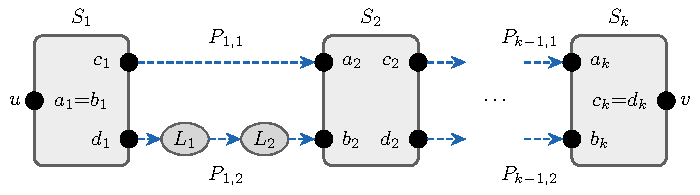
\includegraphics{square-decomposition.pdf}
    \caption{The square decomposition: squares (boxes), links (ellipses) and the directed edges of $F$}
    \label{fig:square-decomposition}
\end{figure}

\begin{example}
\label{ex:decomposition}
In the graph $G_a$ of \cref{ex:counterexamples}, let $p_1 = u, a, t, v$ and $p_2 = u, s, b, v$.
The minimum $u$--$v$ cuts are $\{ua, us\}$, $\{ua, sb\}$, $\{at, bv\}$ and $\{tv, bv\}$, so $F$ contains all edges except $ab$.
The squares are $S_1 = \{u\}$, $S_2 = \{a, b\}$ and $S_3 = \{v\}$, and the links are $\{s\}$ and $\{t\}$ (\cref{fig:decomposition-example}).
The terminals of $S_2$ are $a_2 = c_2 = a$ and $b_2 = d_2 = b$.
The general paths are $P_{1,1} = ua$, $P_{1,2} = us, \{s\}, sb$, $P_{2,1} = at, \{t\}, tv$ and $P_{2,2} = bv$.
\end{example}

\begin{figure}[tb]
    \centering
    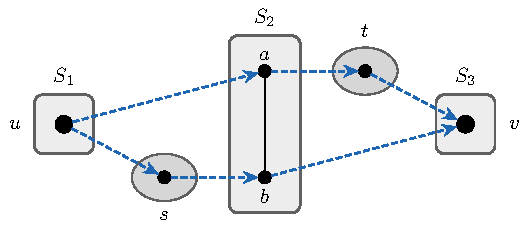
\includegraphics{decomposition-example.pdf}
    \caption{The square decomposition of $G_a$ with respect to $u$ and $v$}
    \label{fig:decomposition-example}
\end{figure}

\begin{example}
\label{ex:worked}
Let $G_1$ be the graph with the vertices $u, v, 1, \dots, 8$ and the edges
\[
u1,\ u2,\ 12,\ 13,\ 23,\ 36,\ 24,\ 45,\ 57,\ 67,\ 68,\ 7v,\ 8v
\]
(\cref{fig:worked-example}).
We have $c(u, v) = 2$ and $d(u, v) = 5$, and we take $p_1 = u, 1, 3, 6, 8, v$ and $p_2 = u, 2, 4, 5, 7, v$.
The minimum $u$--$v$ cuts are $\{u1, u2\}$, $\{36, 24\}$, $\{36, 45\}$, $\{36, 57\}$, $\{68, 7v\}$ and $\{8v, 7v\}$, so $F$ contains all edges except $12$, $13$, $23$ and $67$.
The squares are $S_1 = \{u\}$, $S_2 = \{1, 2, 3\}$, $S_3 = \{6, 7\}$ and $S_4 = \{v\}$, and the links are $\{4\}$, $\{5\}$ and $\{8\}$.
The terminals are $a_2 = 1$, $b_2 = d_2 = 2$, $c_2 = 3$, $a_3 = c_3 = 6$ and $b_3 = d_3 = 7$.
The general paths $P_{1,1}$, $P_{1,2}$, $P_{2,1}$ and $P_{3,2}$ are the single edges $u1$, $u2$, $36$ and $7v$, while $P_{2,2} = 24, \{4\}, 45, \{5\}, 57$ and $P_{3,1} = 68, \{8\}, 8v$.
Every vertex outside $S_2 \cup S_3$ has degree two, two vertices of the same square are adjacent, and the cut $\{36, 24\}$ separates $S_2$ from $S_3$.
Hence $G_1 \in \DC$.
\end{example}

\begin{figure}[tb]
    \centering
    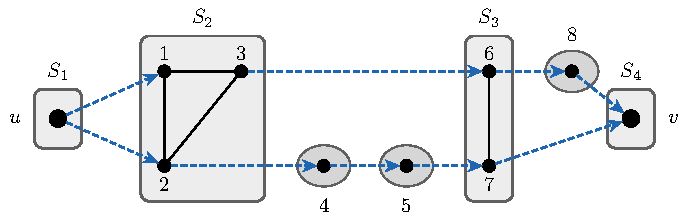
\includegraphics{worked-example.pdf}
    \caption{The graph $G_1$ of \cref{ex:worked} and its square decomposition}
    \label{fig:worked-example}
\end{figure}

\section{Separating Shortest Paths}
\label{sec:separating}

By \cref{lem:basic-bounds} and \cref{prop:easy-pairs}(iii), a pair with $c(u, v) = 2$ satisfies $\cp(u, v) = d(u, v)$ if $G$ contains a separating shortest $u$--$v$ path, and $\cp(u, v) = d(u, v) + 1$ otherwise.
Whether a $u$--$v$ path separates $u$ from $v$ is decided inside the squares.

Let $R$ be a $u$--$v$ path.
By \cref{thm:structure}(ii) and \cref{lem:pieces}(iii), the path $R$ contains exactly one of the two edges that enter $S_i$, for $2 \leq i \leq k$, and exactly one of the two edges that leave $S_i$, for $1 \leq i < k$.
Let $x_i$ be the head of the edge of $R$ that enters $S_i$, and let $\alpha_i$ be the head of the other edge that enters $S_i$.
Let $y_i$ be the tail of the edge of $R$ that leaves $S_i$, and let $\beta_i$ be the tail of the other edge that leaves $S_i$.
We put $x_1 = \alpha_1 = u$ and $y_k = \beta_k = v$.
Then $(x_i, \alpha_i)$ is $(a_i, b_i)$ or $(b_i, a_i)$, the pair $(y_i, \beta_i)$ is $(c_i, d_i)$ or $(d_i, c_i)$, and the trace of $R$ in $S_i$ is an $x_i$--$y_i$ path (\cref{fig:square-terminals}).

\begin{figure}[tb]
    \centering
    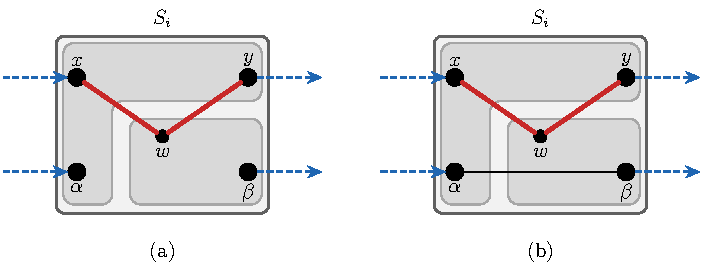
\includegraphics{square-terminals.pdf}
    \caption{A square $S_i$ and a trace $x, w, y$ that separates $\alpha$ from $\beta$ in (a) and does not in (b)}
    \label{fig:square-terminals}
\end{figure}

\begin{lemma}[Separation criterion]
\label{lem:criterion}
Let $c(u, v) = 2$, and let $R$ be a $u$--$v$ path.
The graph $G \setminus R$ contains a $u$--$v$ path if and only if, for every $i \in \{1, \dots, k\}$, the vertices $\alpha_i$ and $\beta_i$ lie in the same component of $S_i \setminus R$.
\end{lemma}

\begin{proof}
Let $1 \leq i < k$.
By \cref{thm:structure}(iv), $R$ contains the edges of one of the general paths from $S_i$ to $S_{i+1}$, and it contains no edge and visits no link of the other one, which we denote by $e_0, L_1, e_1, \dots, L_r, e_r$.
The edge $e_0$ is the edge that leaves $S_i$ and does not lie on $R$, so its tail is $\beta_i$, and likewise the head of $e_r$ is $\alpha_{i+1}$.
The links $L_1, \dots, L_r$ are connected and contain no edge of $R$.
Hence $\beta_i$ and $\alpha_{i+1}$ lie in the same component of $G \setminus R$.

Suppose that $\alpha_i$ and $\beta_i$ lie in the same component of $S_i \setminus R$ for every $i$.
Then $u = \alpha_1$, $\beta_1$, $\alpha_2$, $\beta_2$, \dots, $\alpha_k$, $\beta_k = v$ all lie in the same component of $G \setminus R$.

Conversely, let $Q$ be a $u$--$v$ path of $G \setminus R$, and let $1 \leq i \leq k$.
By \cref{thm:structure}(ii), $Q$ visits $S_i$.
If $i \geq 2$, the path $Q$ contains an edge that enters $S_i$ and does not lie on $R$, so the first vertex of $Q$ in $S_i$ is $\alpha_i$.
If $i = 1$, this vertex is $u = \alpha_1$.
In the same way, the last vertex of $Q$ in $S_i$ is $\beta_i$.
The trace of $Q$ in $S_i$ is therefore an $\alpha_i$--$\beta_i$ path of $S_i \setminus R$.
\end{proof}

\begin{theorem}[Separating shortest paths]
\label{thm:characterization}
Let $G$ be a connected graph, let $u$ and $v$ be two vertices of $G$ with $c(u, v) = 2$, and let $S_1, \dots, S_k$ be the squares of $G$ with respect to $u$ and $v$, with the terminals $a_i, b_i, c_i, d_i$.
Then $\cp(u, v) = d(u, v)$ if and only if there are an index $i$, a pair $(x, \alpha) \in \{(a_i, b_i), (b_i, a_i)\}$, a pair $(y, \beta) \in \{(c_i, d_i), (d_i, c_i)\}$ and an $x$--$y$ path $p$ of $S_i$ such that
(i) $d(u, x) + |p| + d(y, v) = d(u, v)$ and
(ii) the vertices $\alpha$ and $\beta$ lie in different components of $S_i \setminus p$.
Otherwise $\cp(u, v) = d(u, v) + 1$.
\end{theorem}

\begin{proof}
Suppose that $i$, $(x, \alpha)$, $(y, \beta)$ and $p$ satisfy (i) and (ii).
Let $R_x$ be a shortest $u$--$x$ path and let $R_y$ be a shortest $y$--$v$ path of $G$.
By (i), the paths $R_x$, $p$ and $R_y$ form a walk from $u$ to $v$ with $d(u, v)$ edges.
Such a walk repeats no vertex, so it is a shortest $u$--$v$ path $R$.
Let $x_i, \alpha_i, y_i, \beta_i$ be defined for $R$ as above, and let $p'$ be the trace of $R$ in $S_i$, which contains $p$.
We show that $\alpha_i$ and $\alpha$ lie in the same component of $S_i \setminus p$.
This holds if $\alpha_i = \alpha$, in particular if $i = 1$.
Otherwise $(x_i, \alpha_i) = (\alpha, x)$, and the part of $p'$ from $x_i = \alpha$ to $x$ is a path of $S_i$ that shares no edge with $p$ and joins $\alpha$ to $\alpha_i = x$.
In the same way, $\beta_i$ and $\beta$ lie in the same component of $S_i \setminus p$.
By (ii), the vertices $\alpha_i$ and $\beta_i$ lie in different components of $S_i \setminus p$, and hence of its subgraph $S_i \setminus R$.
By \cref{lem:criterion}, $R$ is a separating shortest $u$--$v$ path, and $\cp(u, v) = d(u, v)$ by \cref{lem:basic-bounds}.

Conversely, suppose that $\cp(u, v) = d(u, v)$.
By \cref{lem:basic-bounds}, $G$ contains a separating shortest $u$--$v$ path $R$, and by \cref{lem:criterion}, the vertices $\alpha_i$ and $\beta_i$ lie in different components of $S_i \setminus R$ for some $i$.
Let $p$ be the trace of $R$ in $S_i$, and let $(x, \alpha) = (x_i, \alpha_i)$ and $(y, \beta) = (y_i, \beta_i)$.
Condition (ii) holds because $S_i \setminus R = S_i \setminus p$.
Condition (i) holds because the parts of the shortest path $R$ from $u$ to $x$ and from $y$ to $v$ are shortest paths.

The last statement follows from \cref{prop:easy-pairs}(iii).
\end{proof}

A path $p$ with (i) is a shortest $x$--$y$ path of $G$, because $d(u, v) \leq d(u, x) + d(x, y) + d(y, v)$.
A path $p$ with (ii) has at least one edge, because $S_i$ is connected.
The first part of the proof constructs a separating shortest $u$--$v$ path from $p$.

\begin{example}
\label{ex:criterion}
In the graph $G_a$ (\cref{ex:decomposition}), take $i = 2$, $(x, \alpha) = (a, b)$, $(y, \beta) = (b, a)$ and $p = a, b$.
Then $d(u, a) + |p| + d(b, v) = 3 = d(u, v)$, and the graph $S_2 \setminus p$ has no edge, so it separates $\alpha = b$ from $\beta = a$.
Hence $\cp(u, v) = 3$.

In the graph $G_1$ (\cref{ex:worked}), take $i = 3$, $(x, \alpha) = (6, 7)$, $(y, \beta) = (7, 6)$ and $p = 6, 7$.
Then $d(u, 6) + |p| + d(7, v) = 3 + 1 + 1 = d(u, v)$, and $S_3 \setminus p$ has no edge.
Hence $\cp(u, v) = 5$, and $u, 1, 3, 6, 7, v$ is a minimum cut-path.

Let $G_1'$ be obtained from $G_1$ by adding a vertex $9$ adjacent to $6$ and $7$.
The set $F$, the distances from $u$ and to $v$ and the squares $S_1, S_2, S_4$ do not change, and $S_3 = \{6, 7, 9\}$.
The only paths with at least one edge that satisfy (i) are the edges $13$ and $23$ of $S_2$ and the edge $67$ of $S_3$, and each of the graphs $S_2 \setminus \{13\}$, $S_2 \setminus \{23\}$ and $S_3 \setminus \{67\}$ is connected.
Hence $\cp(u, v) = 6$ in $G_1'$.

Let $G_1''$ be obtained from $G_1$ by removing the vertex $5$ and adding the edge $47$.
Then $d(u, v) = 4$, the squares are those of $G_1$, and no path of a square with at least one edge satisfies (i).
Hence $\cp(u, v) = 5$ in $G_1''$.
\end{example}

Condition (i) of \cref{thm:characterization} refers to distances in $G$.
If the trace of a $u$--$v$ path in a square and the edges by which the path enters and leaves the square are prescribed, the minimum length of such a path is given by two distances in a directed graph (\cref{prop:lengths}).
Let $\vec{G}$ be obtained from $G$ by directing every edge of $F$ from its tail to its head.
A \emph{directed path} of $\vec{G}$ is a path of $G$ that traverses every edge of $F$ from its tail to its head.
For an edge $e \in F$ with the tail $s$ and the head $t$, let $\lambda^{-}(e)$ be the minimum number of edges of a directed $u$--$s$ path and let $\lambda^{+}(e)$ be the minimum number of edges of a directed $t$--$v$ path of $\vec{G}$.

\begin{proposition}
\label{prop:lengths}
Let $c(u, v) = 2$.
(i) The $u$--$v$ paths of $G$ are exactly the directed $u$--$v$ paths of $\vec{G}$.
(ii) Let $1 < i < k$, let $g$ be an edge that enters $S_i$, let $h$ be an edge that leaves $S_i$, and let $p$ be a path of $S_i$ from the head of $g$ to the tail of $h$.
Then the minimum number of edges of a $u$--$v$ path that contains $g$ and $h$ and has the trace $p$ in $S_i$ is
\[
\lambda^{-}(g) + |p| + \lambda^{+}(h) + 2.
\]
For $i = 1$ and a path $p$ of $S_1$ from $u$ to the tail of $h$, the minimum over the $u$--$v$ paths that contain $h$ and have the trace $p$ in $S_1$ is $|p| + \lambda^{+}(h) + 1$.
For $i = k$ and a path $p$ of $S_k$ from the head of $g$ to $v$, the corresponding minimum is $\lambda^{-}(g) + |p| + 1$.
\end{proposition}

\begin{proof}
(i) This is \cref{lem:orientation}(iii).

(ii) Let $1 < i < k$, let $s$ be the tail of $g$ and let $t$ be the head of $h$.
A $u$--$v$ path that contains $g$ and $h$ and has the trace $p$ in $S_i$ consists of a $u$--$s$ path, the edge $g$, the path $p$, the edge $h$ and a $t$--$v$ path.
By (i), the first and the last part are directed paths, so the path has at least $\lambda^{-}(g) + |p| + \lambda^{+}(h) + 2$ edges.
For the converse, let $R^{-}$ be a shortest directed $u$--$s$ path and let $R^{+}$ be a shortest directed $t$--$v$ path.
Let $\delta(A)$ and $\delta(B)$ be the minimum $u$--$v$ cuts formed by the edges that enter $S_i$ and by the edges that leave $S_i$ (\cref{thm:structure}(i)).
The set $S_i$ is disjoint from $A$ and contained in $B$.
The edges of $\delta(A)$ have their tails in $A$, so no directed path leads from a vertex outside $A$ to a vertex of $A$, and the same holds for $B$.
Since $s \in A$, all vertices of $R^{-}$ lie in $A$.
Both ends of $h$ lie outside $A$, because $h \notin \delta(A)$, and $t \notin B$.
Hence all vertices of $R^{+}$ lie outside $A \cup B$.
The sets $A$, $S_i$ and $V \setminus (A \cup B)$ are pairwise disjoint, so $R^{-}$, $g$, $p$, $h$ and $R^{+}$ form a $u$--$v$ path with the trace $p$ in $S_i$ and with $\lambda^{-}(g) + |p| + \lambda^{+}(h) + 2$ edges.
For $i = 1$ the parts $R^{-}$ and $g$ are omitted, and for $i = k$ the parts $h$ and $R^{+}$.
\end{proof}

By \cref{prop:lengths} and \cref{lem:criterion}, \cref{thm:characterization} remains true if condition (i) is replaced by $\lambda^{-}(g) + |p| + \lambda^{+}(h) + 2 = d(u, v)$.
Here $g$ and $h$ are edges that enter and leave $S_i$, the path $p$ leads from the head of $g$ to the tail of $h$, and $\alpha$ and $\beta$ are the head and the tail of the other entering and leaving edge.
For $i = 1$ and $i = k$, the sum is changed as in \cref{prop:lengths}.
Indeed, by \cref{prop:lengths} the equation holds if and only if some shortest $u$--$v$ path contains $g$ and $h$ and has the trace $p$ in $S_i$, and for such a path $\alpha_i = \alpha$ and $\beta_i = \beta$, so \cref{lem:criterion} applies.

\section{A Linear-Time Algorithm}
\label{sec:algorithm}

In a graph of $\DC$, the paths $p$ of \cref{thm:characterization} have at most two edges, and a constant number of them has to be tested in each square.

\begin{corollary}
\label{cor:two-edges}
Let $G \in \DC$ and let $u, v$ be two vertices of $G$ with $c(u, v) = 2$.
Then every shortest $u$--$v$ path has at most two edges in every square.
Every path $p$ that satisfies condition (i) of \cref{thm:characterization} has $|p| = d(x, y) \leq 2$.
\end{corollary}

\begin{proof}
Let $x$ be an entering terminal and let $y$ be a leaving terminal of a square $S_i$.
If $x \neq y$, then $c(x, y) \geq 3$ by \cref{thm:structure}(v), and $d(x, y) \leq 2$ by \cref{def:class}.
Hence $d(x, y) \leq 2$ in all cases.
The trace of a shortest $u$--$v$ path in $S_i$ is a shortest path of $G$ from an entering terminal to a leaving terminal of $S_i$.
It contains all edges of the path in $S_i$, because an edge of a path joins two consecutive vertices of the path.
A path $p$ with (i) is a shortest $x$--$y$ path of $G$.
\end{proof}

The set $F$ is computed from $p_1$ and $p_2$.
Let $D$ be the directed graph with the vertex set $V$ that contains, for every edge $xy$ of $G$ outside $p_1 \cup p_2$, the arcs from $x$ to $y$ and from $y$ to $x$, and for every edge $xy$ that $p_1$ or $p_2$ traverses from $x$ to $y$, the arc from $y$ to $x$.
It is the residual graph of the flow that sends one unit along $p_1$ and one along $p_2$.
For a directed network, statement (i) of the following lemma is the theorem of Picard and Queyranne~\cite{PicardQueyranne1980} on the closed sets of the residual graph of a maximum flow, and statement (ii) is their criterion for saturated arcs.
We give the short proofs for the flow of value two in the undirected graph $G$, where every edge outside $p_1 \cup p_2$ has both arcs in $D$.

\begin{lemma}
\label{lem:residual}
Let $c(u, v) = 2$.
(i) For a set $A \subseteq V$ with $u \in A$ and $v \notin A$, the set $\delta(A)$ is a minimum $u$--$v$ cut if and only if no arc of $D$ leads from $A$ to $V \setminus A$.
(ii) An edge $xy$ that $p_1$ or $p_2$ traverses from $x$ to $y$ belongs to $F$ if and only if $x$ and $y$ lie in different strong components of $D$.
\end{lemma}

\begin{proof}
(i) Let $\delta(A)$ be a minimum $u$--$v$ cut.
By \cref{lem:orientation}, it consists of an edge of $p_1$ and an edge of $p_2$, and each of them is traversed by its path from $A$ to $V \setminus A$.
The arcs of these two edges lead into $A$, and no other arc has its ends on different sides.
Conversely, suppose that no arc of $D$ leads from $A$ to $V \setminus A$.
Then every edge of $\delta(A)$ lies on $p_1$ or $p_2$ and is traversed by its path from $A$ to $V \setminus A$.
A path that starts in $A$ and has left $A$ cannot leave $A$ again without returning to $A$ first, so each of $p_1$ and $p_2$ contains exactly one edge of $\delta(A)$.
Hence $\delta(A)$ is a $u$--$v$ cut with two edges.

(ii) Let $p_j$ be the path that contains $xy$.
If $xy \in F$, it lies in a minimum $u$--$v$ cut $\delta(A)$, and $x \in A$, $y \notin A$ by \cref{lem:orientation}(ii).
By (i), no directed path of $D$ leads from $x$ to $y$, so $x$ and $y$ lie in different strong components.
Conversely, suppose that $x$ and $y$ lie in different strong components.
Since $D$ contains the arc from $y$ to $x$, no directed path of $D$ leads from $x$ to $y$.
Let $A$ be the set of all vertices that can be reached from $x$ by directed paths of $D$.
Then $x \in A$, $y \notin A$, and no arc leads from $A$ to $V \setminus A$.
The arcs of the edges of $p_j$ form a directed path from $v$ through $y$ and $x$ to $u$.
Hence $u \in A$, and $v \notin A$ because $y$ can be reached from $v$.
By (i), $\delta(A)$ is a minimum $u$--$v$ cut, and it contains $xy$.
\end{proof}

\begin{algorithm}[tb]
\caption{A minimum cut-path if $c(u, v) = 2$, or two vertices that show $G \notin \DC$}
\label{alg:cut-two}
\begin{algorithmic}[1]
\Require a connected graph $G = (V, E)$ and two vertices $u, v$ with $c(u, v) = 2$
\Ensure $\cp(u, v)$ and a minimum cut-path between $u$ and $v$, or two vertices $x, y$ with $c(x, y) \geq 3$ and $d(x, y) \geq 3$ and a cut-path between $u$ and $v$ with $d(u, v) + 1$ edges
\State compute $d(u, z)$ and $d(z, v)$ for all $z \in V$ by two breadth-first searches \label{line:bfs}
\State compute two edge-disjoint $u$--$v$ paths $p_1$ and $p_2$ \label{line:paths}
\State $F \gets$ the edges of $p_1 \cup p_2$ whose ends lie in different strong components of $D$ \label{line:residual}
\State compute the pieces, the squares $S_1, \dots, S_k$ and their terminals \label{line:pieces}
\For{$i \gets 1$ to $k$} \label{line:loop}
    \For{each $(x, \alpha) \in \{(a_i, b_i), (b_i, a_i)\}$ and $(y, \beta) \in \{(c_i, d_i), (d_i, c_i)\}$ with $x \neq y$ and $\alpha \neq \beta$}
        \State $\ell \gets d(u, v) - d(u, x) - d(y, v)$ \label{line:length}
        \If{$\ell \geq 3$}
            \State record the pair $x, y$ \Comment{$c(x, y) \geq 3$ and $d(x, y) \geq 3$} \label{line:record}
        \EndIf
        \State $\mathcal{P} \gets \emptyset$
        \If{$\ell = 1$ and $xy \in E$}
            \State $\mathcal{P} \gets$ the set that contains the path $x, y$ \label{line:edge}
        \ElsIf{$\ell = 2$}
            \State $q \gets$ an $\alpha$--$\beta$ path of $S_i$ \label{line:q}
            \State $\mathcal{P} \gets$ the set of the paths $x, w, y$ of $S_i$ such that $xw$ or $wy$ is an edge of $q$ \label{line:candidates}
        \EndIf
        \For{each $p \in \mathcal{P}$}
            \If{$\alpha$ and $\beta$ lie in different components of $S_i \setminus p$} \label{line:test}
                \State \Return $d(u, v)$ and $R_x \cup p \cup R_y$ for a shortest $u$--$x$ path $R_x$ and a shortest $y$--$v$ path $R_y$ \label{line:found}
            \EndIf
        \EndFor
    \EndFor
\EndFor
\State $R \gets$ a shortest $u$--$v$ path, $C \gets$ the set of the two edges that leave $S_1$ \label{line:union}
\If{a pair $x, y$ is recorded}
    \State \Return $x, y$ and $R \cup C$ \label{line:certificate}
\EndIf
\State \Return $d(u, v) + 1$ and $R \cup C$ \label{line:not-found}
\end{algorithmic}
\end{algorithm}

\Cref{alg:cut-two} computes the square decomposition and searches every square for a path $p$ as in \cref{thm:characterization} with at most two edges.
For a path with two edges it uses that a path which separates $\alpha$ from $\beta$ shares an edge with every $\alpha$--$\beta$ path of the square.
The algorithm does not test whether $G \in \DC$.

\begin{theorem}
\label{thm:linear-time}
There is an algorithm that, given a connected graph $G = (V, E)$ and two distinct vertices $u, v$ of $G$, decides in $O(|V| + |E|)$ time whether $c(u, v) \leq 2$.
If so, it returns within the same time $\cp(u, v)$ and a minimum cut-path between $u$ and $v$, or it returns two vertices $x, y$ with $c(x, y) \geq 3$ and $d(x, y) \geq 3$, which show that $G \notin \DC$, and a cut-path between $u$ and $v$ with $d(u, v) + 1 \leq \cp(u, v) + 1$ edges.
The second outcome does not occur for $G \in \DC$.
\end{theorem}

\begin{proof}
The algorithm first computes, by at most three augmentations of the algorithm of Ford and Fulkerson~\cite[Section~10.4]{Erickson2019Algorithms}, a flow from $u$ to $v$ of value at most three in which every edge of $G$ carries at most one unit.
Each augmentation is a search in the residual graph of the current flow and takes $O(|V| + |E|)$ time.
The first augmentation succeeds because $G$ is connected.
The cut-value $c(u, v)$ is one if the second augmentation fails, two if the third one fails, and at least three otherwise.
If $c(u, v) = 1$, the algorithm returns $d(u, v)$ and a shortest $u$--$v$ path, which is correct by \cref{prop:easy-pairs}(ii).

Let $c(u, v) = 2$.
The two augmenting paths need not be edge-disjoint, because the second one can traverse an edge of the first one backwards, which cancels the flow on this edge.
The paths $p_1$ and $p_2$ are therefore read from the flow of value two.
Let $H$ be the directed graph formed by the edges that carry flow, each directed along the flow.
In $H$, the vertex $u$ has two more leaving than entering arcs, the vertex $v$ has two more entering than leaving arcs, and every other vertex has as many entering as leaving arcs.
No arc of $H$ leaves the set $X$ of the vertices that can be reached from $u$, so the vertices of $X$ have in total at most as many leaving as entering arcs, and hence $v \in X$.
A search in $H$ therefore finds a $u$--$v$ path $p_1$.
After the removal of the arcs of $p_1$, the same argument with one in place of two gives a $u$--$v$ path $p_2$.
The paths $p_1$ and $p_2$ are edge-disjoint paths of $G$, and the arcs of $H$ that remain form cycles and are not used.
Line~\ref{line:paths} of \cref{alg:cut-two} takes these two paths, and the algorithm runs \cref{alg:cut-two}.

\emph{Correctness.}
By \cref{lem:residual}(ii), line~\ref{line:residual} computes the set $F$, and the direction in which $p_1$ or $p_2$ traverses an edge of $F$ gives its tail and its head.
Line~\ref{line:pieces} therefore computes the squares and the terminals of \cref{def:pieces,def:decomposition}.
Every path $p$ that is tested in line~\ref{line:test} is an $x$--$y$ path of $S_i$ with $\ell$ edges, so it satisfies condition (i) of \cref{thm:characterization}.
If the test succeeds, $p$ also satisfies condition (ii).
By the proof of \cref{thm:characterization}, the set returned in line~\ref{line:found} is then a separating shortest $u$--$v$ path, which is a cut-path with $d(u, v) = \cp(u, v)$ edges.
A path returned in line~\ref{line:found} is thus a minimum cut-path in every connected graph.

If line~\ref{line:length} gives $\ell \geq 3$ for two terminals $x \neq y$, then $d(x, y) \geq \ell \geq 3$, because $d(u, v) \leq d(u, x) + d(x, y) + d(y, v)$, and $c(x, y) \geq 3$ by \cref{thm:structure}(v).
A pair recorded in line~\ref{line:record} therefore shows that $G \notin \DC$, and no pair is recorded if $G \in \DC$.

Suppose now that $\cp(u, v) = d(u, v)$ and that no pair is recorded.
By \cref{thm:characterization}, there are $i$, $(x, \alpha)$, $(y, \beta)$ and $p$ with (i) and (ii).
Then $\alpha \neq \beta$ and the path $p$ has at least one edge, so $x \neq y$, and line~\ref{line:length} gives $\ell = |p|$ for these terminals.
Since the pair $x, y$ is not recorded, $\ell \in \{1, 2\}$.
If $\ell = 1$, then $p$ is the path of line~\ref{line:edge}.
If $\ell = 2$, let $p = x, w, y$.
The path $q$ of line~\ref{line:q} is not a path of $S_i \setminus p$, so it contains the edge $xw$ or the edge $wy$.
In both cases $p \in \mathcal{P}$, so the algorithm returns in line~\ref{line:found}, for this path or for an earlier one.

Hence, if the algorithm reaches line~\ref{line:not-found}, then $\cp(u, v) = d(u, v) + 1$.
The set $C$ of line~\ref{line:union} is a minimum $u$--$v$ cut by \cref{thm:structure}(i), and $R$ contains exactly one of its edges by \cref{lem:orientation}(ii).
Hence $R \cup C$ is a cut-path with $d(u, v) + 1$ edges, which is a minimum cut-path in line~\ref{line:not-found} and has at most $\cp(u, v) + 1$ edges in line~\ref{line:certificate}.

\emph{Running time.}
The graph is given by adjacency lists.
Breadth-first search~\cite[Section~8.4]{Erickson2019Algorithms} and the computation of strong components~\cite{Tarjan1972DFS} take $O(|V| + |E|)$ time.
The paths $p_1$ and $p_2$ are found by two searches in $H$.
Lines~\ref{line:bfs} to~\ref{line:pieces} consist of a constant number of such computations and of one search in $G \setminus F$ for the pieces.
Let $S_i$ have $n_i$ vertices and $m_i$ edges.
For each of the at most four choices of $(x, \alpha)$ and $(y, \beta)$, the path $q$ is found by one search in $S_i$.
The path $q$ has at most two edges at $x$ and at most two edges at $y$, so $\mathcal{P}$ has at most four members.
Whether $x, w, y$ is a path of $S_i$ is decided for each of these vertices $w$ after marking the neighbors of $x$ and of $y$.
A vertex of $S_i$ is an end of at most four edges outside $S_i$, the edges that enter or leave $S_i$, so its neighbors are marked in $O(m_i + 1)$ time.
The test of line~\ref{line:test} is one search in $S_i \setminus p$.
The square $S_i$ therefore takes $O(n_i + m_i)$ time.
The squares are pairwise disjoint, so the loop of line~\ref{line:loop} takes $O(|V| + |E|)$ time.
The paths $R_x$, $R_y$ and $R$ are read from the breadth-first search trees.
\end{proof}

\Cref{alg:cut-two} returns $\cp(u, v)$ and a minimum cut-path whenever no pair is recorded, in particular if every entering terminal of every square is at distance at most two from every leaving terminal of the same square.

\begin{example}
\label{ex:two-edges}
Let $G_a^{+}$ be obtained from the graph $G_a$ of \cref{ex:counterexamples} by adding a vertex $r$ adjacent to $u$ and $b$.
The vertices of degree greater than two are $u$, $a$ and $b$, which are pairwise at distance at most two, so $G_a^{+} \in \DC$.
The minimum $u$--$v$ cuts are $\{at, bv\}$ and $\{tv, bv\}$.
Hence the squares are $S_1 = \{u, s, r, a, b\}$ and $S_2 = \{v\}$, the only link is $\{t\}$, and $c_1 = a$ and $d_1 = b$ for $p_1 = u, a, t, v$.
For $(x, \alpha) = (u, u)$ and $(y, \beta) = (b, a)$, \cref{alg:cut-two} computes $\ell = 3 - 0 - 1 = 2$.
Let $q$ be the path $u, a$.
Its only edge is $ua$, so $w = a$, and $\mathcal{P}$ contains the path $p = u, a, b$.
The vertex $a$ is isolated in $S_1 \setminus p$, so the algorithm returns $3$ and the path $u, a, b, v$.
\end{example}

\begin{corollary}
\label{cor:class-pairs}
Let $G \in \DC$ and let $u, v$ be two distinct vertices of $G$.
If $c(u, v) \leq 2$, in particular if $d(u, v) \geq 3$, then $\cp(u, v)$ and a minimum cut-path between $u$ and $v$ are computed in $O(|V| + |E|)$ time.
If $d(u, v) = 1$, they are computed by one computation of a minimum $u$--$v$ cut.
\end{corollary}

\begin{proof}
A pair with $d(u, v) \geq 3$ has $c(u, v) \leq 2$ by \cref{def:class}.
The first statement is \cref{thm:linear-time}, whose second outcome does not occur for $G \in \DC$, and the second is \cref{prop:easy-pairs}(i).
A minimum $u$--$v$ cut is computed in polynomial time by a maximum flow~\cite[Sections~10.3 and~10.4]{Erickson2019Algorithms}.
\end{proof}

\begin{remark}[Coarser decompositions]
\label{rem:coarser}
Let $F'$ be the union of a nonempty set of minimum $u$--$v$ cuts, and define tails, heads, pieces, squares, links, terminals and general paths with $F'$ in place of $F$.
\Cref{lem:orientation,lem:pieces,lem:degrees}, statements (i) to (iv) of \cref{thm:structure}, \cref{lem:criterion} and \cref{thm:characterization} remain true if \cref{lem:pieces}(i) is restricted to the minimum $u$--$v$ cuts contained in $F'$.
Their proofs use only that every edge of $F$ lies in a minimum $u$--$v$ cut contained in $F$.
Statement (v) of \cref{thm:structure} uses all minimum $u$--$v$ cuts and can fail for $F'$.
If every entering terminal of every square of the coarser decomposition is at distance at most two from every leaving terminal of the same square, then lines~\ref{line:loop} to~\ref{line:not-found} of \cref{alg:cut-two} are correct for this decomposition as well.
The thesis~\cite[Section~3.3]{Michel2025MinCutPath} defines a decomposition into squares and general paths by properties of these subgraphs and constructs one step by step.
The construction starts with one minimum $u$--$v$ cut.
It splits a square, by one of three transformations, only as long as an entering and a leaving terminal of the square are at distance greater than two, so it can stop before all edges of $F$ are removed.
The square decomposition defined here is the finest of the decompositions of this remark.
For $G \in \DC$, it satisfies the distance condition by \cref{thm:structure}(v), and it is a general square graph in the sense of~\cite[Definition~40]{Michel2025MinCutPath}.
\end{remark}

\section{Hardness for Pairs with Cut-Value Two}
\label{sec:hardness}

Without the bound on the distances between terminals, every connected graph $G$ with $c_G(u, v) \geq 3$ occurs as a square with the terminals $u, u, v, v$, and deciding whether it contains a path as in \cref{thm:characterization} is as hard as the \SSP{} problem.

\begin{theorem}
\label{thm:hardness}
It is NP-complete to decide, for a connected graph $G$ and two vertices $u, v$ of $G$ with $c(u, v) = 2$, whether $\cp(u, v) = d(u, v)$.
\end{theorem}

\begin{proof}
By \cref{lem:basic-bounds}, the question is whether $G$ contains a separating shortest $u$--$v$ path.
Such a path is verified in polynomial time by two breadth-first searches, so the problem belongs to NP.

The \SSP{} problem is NP-complete~\cite[Theorem~3.10]{Michel2026MinCutPath}.
For a formula with $n$ variables and $m \geq 1$ clauses, the graph constructed in that reduction contains $2n + 7m \geq 9$ pairwise edge-disjoint $u$--$v$ paths, the threads.
Every $u$--$v$ path lies in the component of $u$, so restricting a graph to this component changes neither its shortest $u$--$v$ paths nor whether one of them is separating.
Hence the problem remains NP-complete for connected graphs $G$ with $c_G(u, v) \geq 3$, and we reduce from this restriction.
Let $G'$ be obtained from such a graph $G$ by adding three new vertices $u', s_1, s_2$ and the edges $u's_1$, $s_1u$, $u's_2$ and $s_2u$ (\cref{fig:padding}).
Every $u'$--$v$ path of $G'$ consists of one of the paths $u', s_1, u$ and $u', s_2, u$ and of a $u$--$v$ path of $G$.
Hence $d_{G'}(u', v) = d_G(u, v) + 2$, and the shortest $u'$--$v$ paths of $G'$ are the paths $R'$ that consist of $u', s_j, u$ for some $j \in \{1, 2\}$ and of a shortest $u$--$v$ path $R$ of $G$.
The two edges at $u'$ form a $u'$--$v$ cut, and $G'$ contains two edge-disjoint $u'$--$v$ paths, so $c_{G'}(u', v) = 2$.
The graph $G' \setminus R'$ consists of $G \setminus R$, of the path $u', s_{3-j}, u$ and of the isolated vertex $s_j$.
It contains a $u'$--$v$ path if and only if $G \setminus R$ contains a $u$--$v$ path.
Therefore $G'$ contains a separating shortest $u'$--$v$ path if and only if $G$ contains a separating shortest $u$--$v$ path.
The graph $G'$ is constructed in polynomial time.
\end{proof}

\begin{figure}[tb]
    \centering
    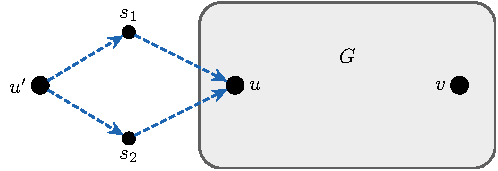
\includegraphics{padding.pdf}
    \caption{The graph $G'$ in the proof of \cref{thm:hardness}; the dashed edges form $F$ if $c_G(u, v) \geq 3$}
    \label{fig:padding}
\end{figure}

Hence the \SSP{} problem remains NP-complete and \MinCutPath{} remains NP-hard for pairs with $c(u, v) = 2$, whereas a shortest $u$--$v$ path solves both for pairs with $c(u, v) = 1$ (\cref{prop:easy-pairs}(ii)).

The square decomposition of $G'$ with respect to $u'$ and $v$ shows where the difficulty lies.
Recall that $c_G(u, v) \geq 3$.
A $u'$--$v$ cut of $G'$ with two edges contains an edge of each of the paths $u', s_1, u$ and $u', s_2, u$, because otherwise it would contain a $u$--$v$ cut of $G$ with at most two edges.
Hence $F$ consists of the four new edges, the squares are $S_1 = \{u'\}$ and $S_2 = V$, and the links are $\{s_1\}$ and $\{s_2\}$.
The terminals of $S_2$ are $a_2 = b_2 = u$ and $c_2 = d_2 = v$, and conditions (i) and (ii) of \cref{thm:characterization} for $S_2$ ask for a separating shortest $u$--$v$ path of $G$.
If $c_G(u, v) = 2$, the four new edges still belong to $F$, but so do the minimum $u$--$v$ cuts of $G$, and $G$ is divided further.

\section{Pairs at Distance Two}
\label{sec:distance-two}

For a graph of $\DC$, \cref{cor:class-pairs} leaves the pairs with $d(u, v) = 2$ and $c(u, v) \geq 3$.
By \cref{prop:easy-pairs}(iv), such a pair has $\cp(u, v) \in \{c(u, v), c(u, v) + 1\}$.

\begin{proposition}
\label{prop:open-pairs}
Let $G$ be a connected graph and let $u, v$ be two distinct vertices of $G$.
Then $\cp(u, v) = c(u, v)$ if and only if some minimum $u$--$v$ cut contains a $u$--$v$ path.
Such a path has an odd number of edges, and at least three edges if $d(u, v) = 2$.
\end{proposition}

\begin{proof}
A minimum $u$--$v$ cut that contains a $u$--$v$ path is a cut-path with $c(u, v)$ edges, and $\cp(u, v) \geq c(u, v)$ by \cref{lem:basic-bounds}.
Conversely, a cut-path with $c(u, v)$ edges contains a $u$--$v$ cut, which has at least $c(u, v)$ edges.
The cut-path is therefore equal to this cut, so it is a minimum $u$--$v$ cut, and it contains a $u$--$v$ path.
A minimum $u$--$v$ cut is $\delta(A)$ for a set $A$ with $u \in A$ and $v \notin A$, and a $u$--$v$ path contained in $\delta(A)$ has an odd number of edges by \cref{lem:minimum-cuts}.
If $d(u, v) = 2$, the path has at least two edges, hence at least three.
\end{proof}

In the graph $G_b$ of \cref{ex:counterexamples}, the minimum $u$--$v$ cut $\delta(\{u, s, b\}) = \{ua, ab, bv\}$ is the path $u, a, b, v$.
In a graph of diameter two, $\cp(u, v) = c(u, v) + 1$ for every pair with $d(u, v) = 2$~\cite[Theorem~15]{Michel2025MinCutPath}, so by \cref{prop:open-pairs} no minimum $u$--$v$ cut contains a $u$--$v$ path.
We do not know a polynomial-time algorithm that computes $\cp(u, v)$ for graphs of $\DC$ and pairs with $d(u, v) = 2$ and $c(u, v) \geq 3$.

\section{Conclusion}\label{sec:conclusion}

In a graph $G = (V, E)$ of $\DC$, a minimum cut-path is computed in $O(|V| + |E|)$ time for every pair with $c(u, v) \leq 2$, which includes every pair with $d(u, v) \geq 3$ (\cref{thm:linear-time}), and by one computation of a minimum $u$--$v$ cut for every pair with $d(u, v) = 1$ (\cref{cor:class-pairs}).
The bound $c(u, v) = 2$ alone does not suffice.
The criterion of \cref{thm:characterization} holds in every graph, but every connected graph with a pair of cut-value at least three occurs as a square, and deciding whether a square contains a path as in the criterion is NP-complete (\cref{thm:hardness}).
In $\DC$, distinct terminals of a square are at distance at most two, so such a path has at most two edges.
Outside $\DC$, the algorithm of \cref{thm:linear-time} either still returns a minimum cut-path or returns two terminals at distance at least three.
For a pair with $d(u, v) = 2$ and $c(u, v) \geq 3$, we know only that $\cp(u, v) \in \{c(u, v), c(u, v) + 1\}$ and that the smaller value is attained if and only if some minimum $u$--$v$ cut contains a $u$--$v$ path (\cref{prop:open-pairs}).

We leave the following questions open.
\begin{enumerate}
\item Can $\cp(u, v)$ be computed in polynomial time for a graph of $\DC$ and a pair with $d(u, v) = 2$ and $c(u, v) \geq 3$?

\item Let $k \geq 3$ be a fixed integer, and consider the connected graphs in which every two distinct vertices $x$ and $y$ satisfy $d(x, y) \leq k$ or $c(x, y) \leq 2$.
Can $\cp(u, v)$ be computed in linear time for the pairs with $c(u, v) = 2$ in these graphs?
The paths of \cref{thm:characterization} then have at most $k$ edges, by the argument of \cref{cor:two-edges}, but the bound of four candidates per pair of terminals in \cref{alg:cut-two} uses that they have at most two.

\item Consider the connected graphs in which every two distinct vertices $x$ and $y$ satisfy $d(x, y) \leq 2$ or $c(x, y) \leq 3$.
Can $\cp(u, v)$ be computed in polynomial time for the pairs with $c(u, v) = 3$ in these graphs?
By \cref{lem:basic-bounds}, such a pair with $d(u, v) \geq 3$ has $d(u, v) \leq \cp(u, v) \leq d(u, v) + 2$, and the square decomposition is defined for cut-value two only.
\end{enumerate}

\backmatter

\bmhead{Acknowledgements}

The idea of the \MinCutPath{} problem is due to Martin Loebl, who supervised the master's thesis on which this paper is based.

\section*{Declarations}

\begin{itemize}
\item Funding: Statement.
\item Conflict of interest/Competing interests: Statement.
\item Ethics approval and consent to participate: Not applicable.
\item Consent for publication: Not applicable.
\item Data availability: No datasets were generated or analyzed during the current study.
\item Materials availability: Not applicable.
\item Code availability: Not applicable.
\item Author contribution: Statement.
\end{itemize}

%%===========================================================================================%%
%% If you are submitting to one of the Nature Portfolio journals, using the eJP submission   %%
%% system, please include the references within the manuscript file itself. You may do this  %%
%% by copying the reference list from your .bbl file, paste it into the main manuscript .tex %%
%% file, and delete the associated \verb+\bibliography+ commands.                            %%
%%===========================================================================================%%

\bibliography{references}% common bib file
%% if required, the content of .bbl file can be included here once bbl is generated
%%\input sn-article.bbl

\end{document}
